\begin{figure}[t]

\begin{minipage}[b]{0.50\linewidth}

{\centering 

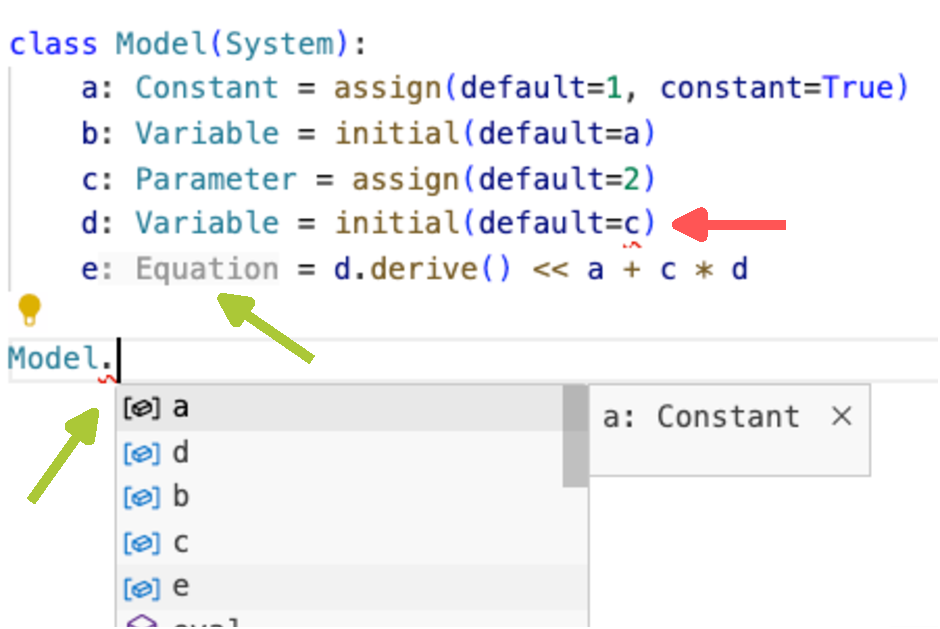
\includegraphics{src/ide/ide1.pdf}

}

\end{minipage}%
%
\begin{minipage}[b]{0.50\linewidth}

{\centering 

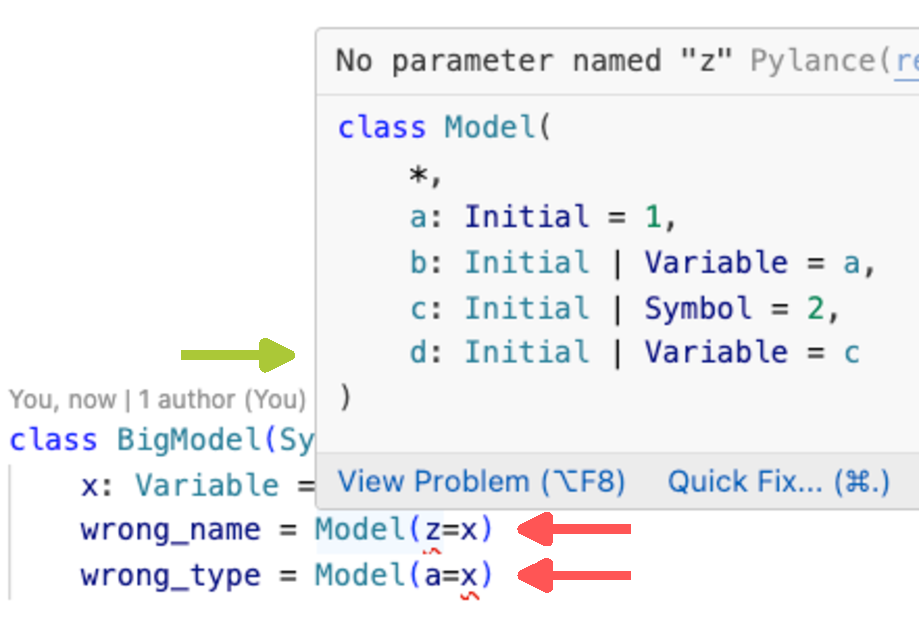
\includegraphics{src/ide/ide2.pdf}

}

\end{minipage}%

\caption{\label{fig-ide}Screenshots of Visual Studio Code showing
tooltips and highlighted type errors. \texttt{Constant} are assigned
with \texttt{assign(...,\ constant=True)} and can be used to link
\texttt{Variable}s initial conditions, while trying to use a
\texttt{Parameter} instead is flagged as type errors (red underlining).
The IDE automatically recognizes \texttt{e} as an \texttt{Equation}, and
provides autocompletion of the variables. A tooltip is shown when
composing models, which show the expected variables and their default
values. The IDE highlights wrong names (\texttt{z} is not a name in
\texttt{Model}) and mismatched types (\texttt{x} is \texttt{Variable}
and \texttt{a} must be a number or a \texttt{Constant})}

\end{figure}
